\documentclass{standalone}
\usepackage{tikz}
\usetikzlibrary{patterns}
\usetikzlibrary{positioning}
\usetikzlibrary{patterns, positioning}
\usetikzlibrary{shapes.misc}
\usepackage[outline]{contour}
\contourlength{1.5pt} 
\usepackage[sfdefault]{ClearSans}

\begin{document}
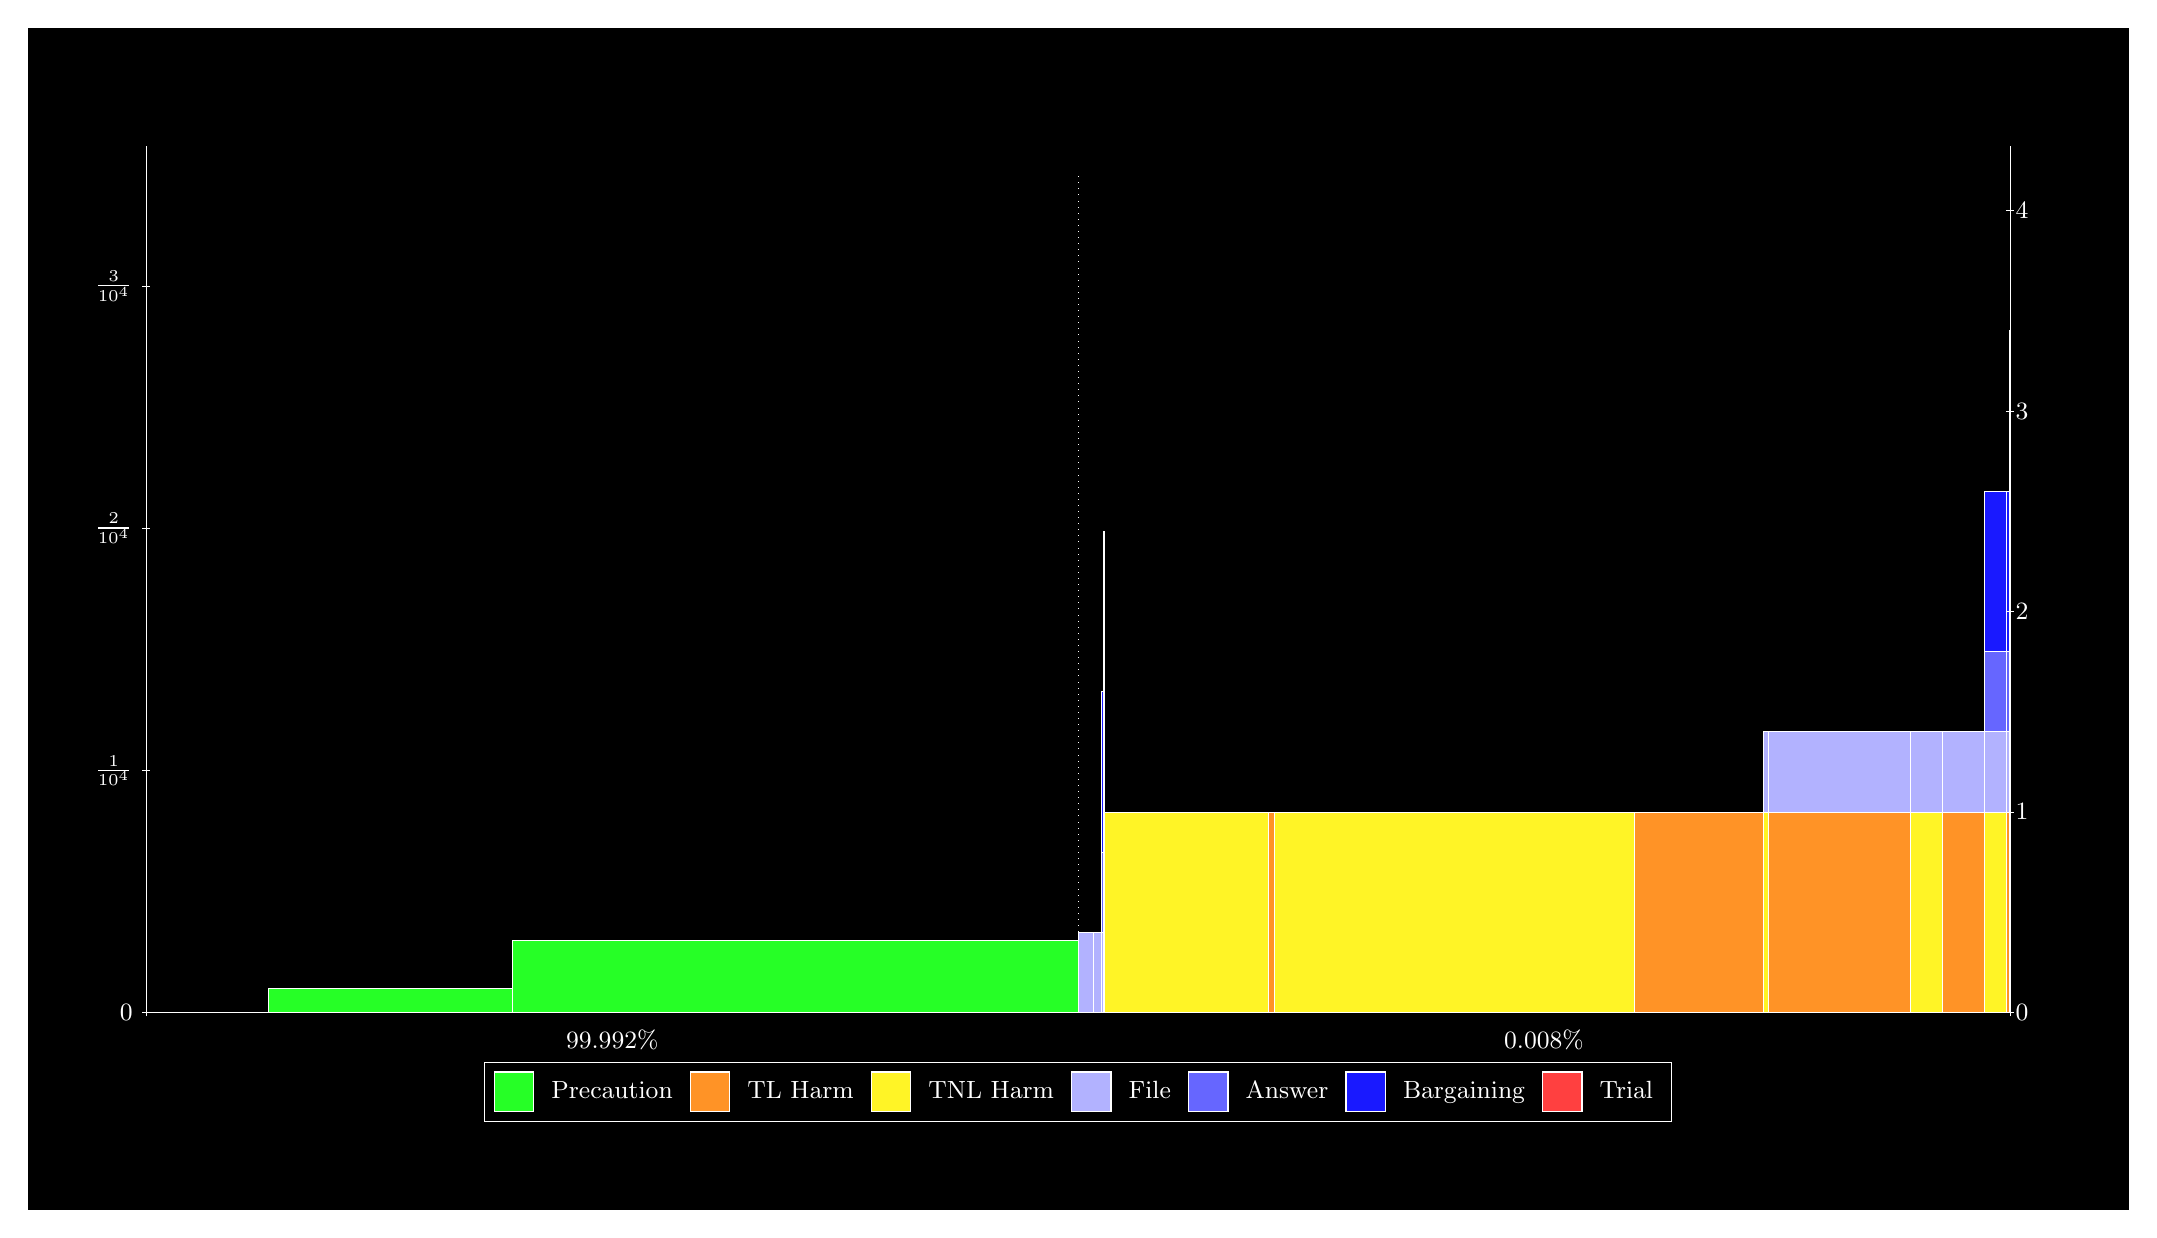
\begin{tikzpicture}
\draw[fill=black] (0,0) rectangle (26.667,15);
\draw[fill=green!85,draw=white,very thin] (3.0469,2.5) rectangle (6.144,2.8075);
\draw[fill=green!85,draw=white,very thin] (6.144,2.5) rectangle (13.333,3.4224);
\draw[fill=blue!30,draw=white,very thin] (13.333,2.5) rectangle (13.52,3.5186);
\draw[fill=green!85,draw=white,very thin] (13.52,2.5) rectangle (13.624,2.5);
\draw[fill=blue!30,draw=white,very thin] (13.52,2.5) rectangle (13.624,3.5186);
\draw[fill=green!85,draw=white,very thin] (13.624,2.5) rectangle (13.659,2.5);
\draw[fill=blue!30,draw=white,very thin] (13.624,2.5) rectangle (13.659,3.5186);
\draw[fill=blue!60,draw=white,very thin] (13.624,3.5186) rectangle (13.659,4.5372);
\draw[fill=blue!90,draw=white,very thin] (13.624,4.5372) rectangle (13.659,6.5744);
\draw[fill=green!85,draw=white,very thin] (13.659,2.5) rectangle (13.66,2.5);
\draw[fill=blue!30,draw=white,very thin] (13.659,2.5) rectangle (13.66,3.5186);
\draw[fill=blue!60,draw=white,very thin] (13.659,3.5186) rectangle (13.66,4.5372);
\draw[fill=blue!90,draw=white,very thin] (13.659,4.5372) rectangle (13.66,6.5744);
\draw[fill=red!75,draw=white,very thin] (13.659,6.5744) rectangle (13.66,8.6116);
\draw[fill=green!85,draw=white,very thin] (13.66,2.5) rectangle (15.745,2.5);
\draw[fill=yellow!85,draw=white,very thin] (13.66,2.5) rectangle (15.745,5.0465);
\draw[fill=green!85,draw=white,very thin] (15.745,2.5) rectangle (15.822,2.5);
\draw[fill=orange!85,draw=white,very thin] (15.745,2.5) rectangle (15.822,5.0465);
\draw[fill=green!85,draw=white,very thin] (15.822,2.5) rectangle (20.391,2.5001);
\draw[fill=yellow!85,draw=white,very thin] (15.822,2.5001) rectangle (20.391,5.0465);
\draw[fill=green!85,draw=white,very thin] (20.391,2.5) rectangle (22.039,2.5001);
\draw[fill=orange!85,draw=white,very thin] (20.391,2.5001) rectangle (22.039,5.0465);
\draw[fill=yellow!85,draw=white,very thin] (22.039,2.5) rectangle (22.1,5.0465);
\draw[fill=blue!30,draw=white,very thin] (22.039,5.0465) rectangle (22.1,6.0651);
\draw[fill=orange!85,draw=white,very thin] (22.1,2.5) rectangle (23.907,5.0465);
\draw[fill=blue!30,draw=white,very thin] (22.1,5.0465) rectangle (23.907,6.0651);
\draw[fill=green!85,draw=white,very thin] (23.907,2.5) rectangle (24.312,2.5);
\draw[fill=yellow!85,draw=white,very thin] (23.907,2.5) rectangle (24.312,5.0465);
\draw[fill=blue!30,draw=white,very thin] (23.907,5.0465) rectangle (24.312,6.0651);
\draw[fill=green!85,draw=white,very thin] (24.312,2.5) rectangle (24.841,2.5);
\draw[fill=orange!85,draw=white,very thin] (24.312,2.5) rectangle (24.841,5.0465);
\draw[fill=blue!30,draw=white,very thin] (24.312,5.0465) rectangle (24.841,6.0651);
\draw[fill=green!85,draw=white,very thin] (24.841,2.5) rectangle (25.126,2.5);
\draw[fill=yellow!85,draw=white,very thin] (24.841,2.5) rectangle (25.126,5.0465);
\draw[fill=blue!30,draw=white,very thin] (24.841,5.0465) rectangle (25.126,6.0651);
\draw[fill=blue!60,draw=white,very thin] (24.841,6.0651) rectangle (25.126,7.0837);
\draw[fill=blue!90,draw=white,very thin] (24.841,7.0837) rectangle (25.126,9.1209);
\draw[fill=green!85,draw=white,very thin] (25.126,2.5) rectangle (25.154,2.5);
\draw[fill=orange!85,draw=white,very thin] (25.126,2.5) rectangle (25.154,5.0465);
\draw[fill=blue!30,draw=white,very thin] (25.126,5.0465) rectangle (25.154,6.0651);
\draw[fill=blue!60,draw=white,very thin] (25.126,6.0651) rectangle (25.154,7.0837);
\draw[fill=blue!90,draw=white,very thin] (25.126,7.0837) rectangle (25.154,9.1209);
\draw[fill=green!85,draw=white,very thin] (25.154,2.5) rectangle (25.16,2.5);
\draw[fill=yellow!85,draw=white,very thin] (25.154,2.5) rectangle (25.16,5.0465);
\draw[fill=blue!30,draw=white,very thin] (25.154,5.0465) rectangle (25.16,6.0651);
\draw[fill=blue!60,draw=white,very thin] (25.154,6.0651) rectangle (25.16,7.0837);
\draw[fill=blue!90,draw=white,very thin] (25.154,7.0837) rectangle (25.16,9.1209);
\draw[fill=red!75,draw=white,very thin] (25.154,9.1209) rectangle (25.16,11.158);
\draw[fill=green!85,draw=white,very thin] (25.16,2.5) rectangle (25.167,2.5);
\draw[fill=orange!85,draw=white,very thin] (25.16,2.5) rectangle (25.167,5.0465);
\draw[fill=blue!30,draw=white,very thin] (25.16,5.0465) rectangle (25.167,6.0651);
\draw[fill=blue!60,draw=white,very thin] (25.16,6.0651) rectangle (25.167,7.0837);
\draw[fill=blue!90,draw=white,very thin] (25.16,7.0837) rectangle (25.167,9.1209);
\draw[fill=red!75,draw=white,very thin] (25.16,9.1209) rectangle (25.167,11.158);
\draw[white,very thin] (1.5,2.5) -- (1.5,13.5);
\draw[white,very thin] (1.45,2.5) -- (1.55,2.5);
\node[font=\small,text=white, anchor=east] at (1.45, 2.5) {0};
\draw[white,very thin] (1.45,5.5745) -- (1.55,5.5745);
\node[font=\small,text=white, anchor=east] at (1.45, 5.5745) {$\frac{1}{10^{4}}$};
\draw[white,very thin] (1.45,8.6491) -- (1.55,8.6491);
\node[font=\small,text=white, anchor=east] at (1.45, 8.6491) {$\frac{2}{10^{4}}$};
\draw[white,very thin] (1.45,11.724) -- (1.55,11.724);
\node[font=\small,text=white, anchor=east] at (1.45, 11.724) {$\frac{3}{10^{4}}$};

\draw[white,dotted,very thin] (13.333,2.83) -- (13.333,13.17);
\draw[white,very thin] (25.167,2.5) -- (25.167,13.5);
\draw[white,very thin] (25.117,2.5) -- (25.217,2.5);
\node[font=\small,text=white, anchor=west] at (25.117, 2.5) {0};
\draw[white,very thin] (25.117,5.0465) -- (25.217,5.0465);
\node[font=\small,text=white, anchor=west] at (25.117, 5.0465) {1};
\draw[white,very thin] (25.117,7.5929) -- (25.217,7.5929);
\node[font=\small,text=white, anchor=west] at (25.117, 7.5929) {2};
\draw[white,very thin] (25.117,10.139) -- (25.217,10.139);
\node[font=\small,text=white, anchor=west] at (25.117, 10.139) {3};
\draw[white,very thin] (25.117,12.686) -- (25.217,12.686);
\node[font=\small,text=white, anchor=west] at (25.117, 12.686) {4};

\draw[white,very thin] (1.5,2.5) -- (25.167,2.5);
\draw[white,very thin] (1.5,2.45) -- (1.5,2.55);
\node[font=\small,text=white, anchor=north] at (1.5, 2.45) {};
\draw[white,very thin] (25.167,2.45) -- (25.167,2.55);
\node[font=\small,text=white, anchor=north] at (25.167, 2.45) {};

\node[font=\small,text=white,anchor=south] at (7.4167, 1.9) {99.992\%};
\node[font=\small,text=white,anchor=south] at (19.25, 1.9) {0.008\%};
\draw (13.3333,2.5) node (B) {};
\begin{scope}[align=center]
\matrix[scale=0.5,draw=white,below=0.5cm of B,nodes={draw},column sep=0.1cm]{
\node[rectangle,draw,minimum width=0.5cm,minimum height=0.5cm,fill=green!85]{}; & \node[draw=none,font=\small,text=white]{Precaution}; &
\node[rectangle,draw,minimum width=0.5cm,minimum height=0.5cm,fill=orange!85]{}; & \node[draw=none,font=\small,text=white]{TL Harm}; &
\node[rectangle,draw,minimum width=0.5cm,minimum height=0.5cm,fill=yellow!85]{}; & \node[draw=none,font=\small,text=white]{TNL Harm}; &
\node[rectangle,draw,minimum width=0.5cm,minimum height=0.5cm,fill=blue!30]{}; & \node[draw=none,font=\small,text=white]{File}; &
\node[rectangle,draw,minimum width=0.5cm,minimum height=0.5cm,fill=blue!60]{}; & \node[draw=none,font=\small,text=white]{Answer}; &
\node[rectangle,draw,minimum width=0.5cm,minimum height=0.5cm,fill=blue!90]{}; & \node[draw=none,font=\small,text=white]{Bargaining}; &
\node[rectangle,draw,minimum width=0.5cm,minimum height=0.5cm,fill=red!75]{}; & \node[draw=none,font=\small,text=white]{Trial}; \\\\
};\end{scope}

\end{tikzpicture}
\end{document}